The \texttt{\pkglnk{model.serialization}} package provides the \texttt{\lnk{Serializable}}
interface. Classes implementing this interface may be serialized into a string.

Since serialization in Wavelength is ad hoc by design, no entity is intended to hold
references to objects of type \texttt{\lnk{Serializable}}. It is provided merely to
ensure consistent naming of the \texttt{serialize} method. Deserialization occurs
in the classes providing the specific type (for example \texttt{\hyperref[type:edu.kit.wavelength.client.model.term.LambdaTerm]{LambdaTerm}}
or \texttt{\hyperref[type:edu.kit.wavelength.client.model.library.Libraries]{Libraries}} and its analogons in \texttt{\pkglnk{model.reduction}}
and \texttt{\pkglnk{model.output}}), which can be done, again, due to the ad hoc nature
of serialization, since each class knows which of its components it has serialized.

\begin{figure}[H]
	\centering
	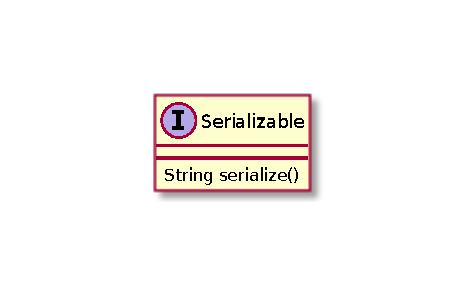
\includegraphics[width=0.35\textwidth]{packageDiagrams/serializationPackage}
\end{figure}
